\section{Implémentation d'un détecteur adaptatif K-CFAR}
\label{sec:kcfar}

Dans le cadre de la détection de cibles dans les images radar à synthèse d'ouverture (SAR), un algorithme de type \textit{Constant False Alarm Rate} (CFAR) a été implémenté. L’objectif de ce type de détecteur est d’adapter dynamiquement le seuil de détection en fonction des statistiques locales du bruit de fond, appelé \textit{clutter}, afin de maintenir une probabilité de fausse alarme constante.

 Dans les images radar, le clutter est caractérisé par un bruit multiplicatif (speckle) et des variations de texture liées à la scène observée. Afin de modéliser ces propriétés, le clutter est ici supposé suivre une distribution K, largement utilisée pour décrire les environnements hétérogènes (mer, terrain urbain, zones naturelles).

\subsection{Modélisation du clutter}

Le clutter radar est modélisé par une distribution statistique non gaussienne, ici en particulier une distribution de type K, adaptée aux environnements hétérogènes. Cette distribution est caractérisée par une intensité moyenne et une variabilité liée à la texture de la scène.

Dans notre implémentation, les paramètres statistiques du clutter sont estimés localement à partir des cellules d’apprentissage. La moyenne et la variance sont définies par :
\begin{equation}
    \mu = \mathbb{E}[I]
\end{equation}
\begin{equation}
    \sigma^2 = \mathrm{Var}(I)
\end{equation}

Ces grandeurs permettent de caractériser le niveau moyen du clutter ainsi que sa dispersion.

\subsection{Principe du détecteur CFAR}

Le détecteur CFAR repose sur l’évaluation d’un seuil adaptatif $T$ pour chaque pixel de l’image. Ce seuil est déterminé de manière à respecter une probabilité de fausse alarme fixée a priori.

La condition de détection s’écrit :
\begin{equation}
    I_{CUT} > T
\end{equation}

où $I_{CUT}$ représente l’intensité du pixel testé (\textit{Cell Under Test}).

Le seuil est calculé sous l’hypothèse que le clutter suit une loi de distribution donnée. Dans ce cas, on impose :
\begin{equation}
    P(I > T \mid H_0) = P_{fa}
\end{equation}

où $H_0$ correspond à l’hypothèse d’absence de cible (clutter seul).

Ainsi, le seuil $T$ est défini comme le quantile de la distribution du clutter :
\begin{equation}
    T = F^{-1}(1 - P_{fa})
\end{equation}

où $F$ est la fonction de répartition du modèle statistique choisi.

\subsection{Structure locale du détecteur}

Pour chaque pixel, une fenêtre glissante est utilisée afin d’estimer localement les statistiques du clutter. Cette fenêtre est composée de trois zones :

\begin{itemize}
    \item la cellule testée (\textit{CUT}),
    \item une zone de garde permettant d’éviter l’influence de la cible sur l’estimation,
    \item une zone d’apprentissage utilisée pour estimer les paramètres statistiques du clutter.
\end{itemize}

Seules les cellules d’apprentissage sont utilisées pour calculer les paramètres statistiques, garantissant ainsi que l’estimation ne soit pas biaisée par la présence d’une cible.

\subsection{Pré-traitement des données}

L’image SAR étant initialement exprimée en amplitude, une conversion en intensité est effectuée. Cette étape est essentielle car les modèles statistiques radar sont définis sur l’intensité du signal.

Une normalisation globale est ensuite appliquée afin de stabiliser les valeurs et rendre les traitements indépendants de l’échelle radiométrique de l’image.

Enfin, un lissage spatial local est appliqué sur le pixel testé afin de réduire l’effet du speckle. Ce lissage permet d’améliorer la robustesse de la décision en diminuant la variance locale du bruit.

\subsection{Calcul du seuil de détection}

Le seuil de détection est déterminé numériquement à partir des paramètres estimés du clutter. L’équation reliant le seuil à la probabilité de fausse alarme ne possédant pas de solution analytique simple dans le cas de la distribution K, une méthode numérique est utilisée.

Dans certains cas particuliers, lorsque les paramètres du clutter indiquent un comportement proche d’une distribution Gamma, une approximation analytique est utilisée afin de réduire le coût de calcul.

Cette étape constitue le cœur du détecteur, car elle permet de garantir que le taux de fausses alarmes reste constant, indépendamment des variations du clutter.

\subsection{Post-traitement spatial}

La carte de détection obtenue après application du CFAR peut contenir des détections isolées dues au bruit speckle. Afin d’améliorer la qualité des résultats, un post-traitement spatial est appliqué.

Ce traitement consiste à :

\begin{itemize}
    \item supprimer les pixels isolés ne présentant pas de cohérence spatiale,
    \item conserver uniquement les zones de détection présentant une structure locale cohérente.
\end{itemize}

Cette étape permet de réduire significativement les fausses alarmes tout en conservant les cibles réelles, qui apparaissent généralement sous forme de structures étendues dans l’image.

\subsection{Validation sur données synthétiques}

Afin de valider le bon fonctionnement du détecteur, des images synthétiques ont été générées, contenant uniquement du clutter ou des cibles ponctuelles insérées artificiellement.
\begin{figure}[htbp]
    \centering
    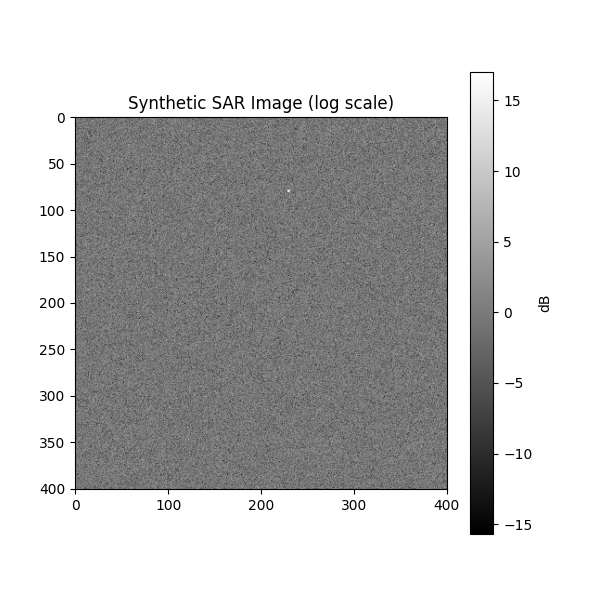
\includegraphics[width=0.6\textwidth, height=0.4\textheight, keepaspectratio]{src/rapport_complet/img/detec_image_synth1.png}
    \caption{Image Synthétique avant application de l'algorithme de détection}
    \label{fig:image_radar_CFAR}
\end{figure}
\begin{figure}[H]
    \centering
    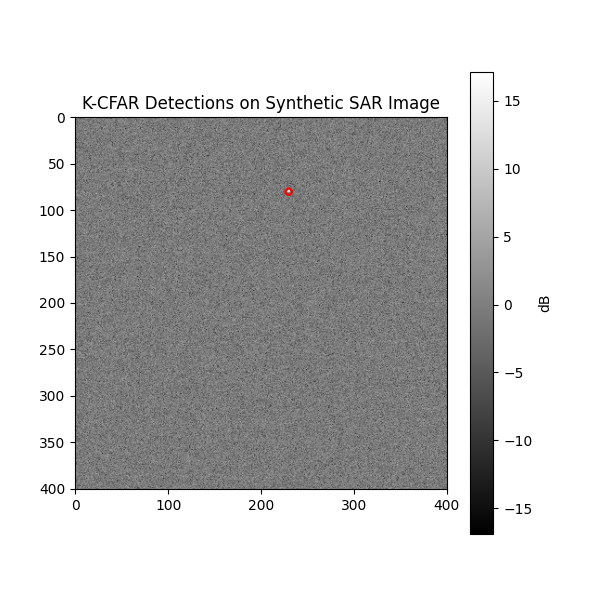
\includegraphics[width=0.6\textwidth, height=0.4\textheight, keepaspectratio]{src/rapport_complet/img/detec_image_synth2.png}
    \caption{Image Synthétique après application de l'algorithme de détection}
    \label{fig:visu_gain_approx_et_reel}
\end{figure}
Ces tests permettent notamment de vérifier que la probabilité de fausse alarme mesurée correspond à la valeur théorique imposée.

\subsection{Validation sur données réelles}

Le détecteur a ensuite été appliqué à des images SAR réelles issues de la base UAVSAR. Afin de limiter le coût de calcul, les images ont été découpées en sous-images de taille $128 \times 128$ pixels.
\begin{figure}[htbp]
    \centering
    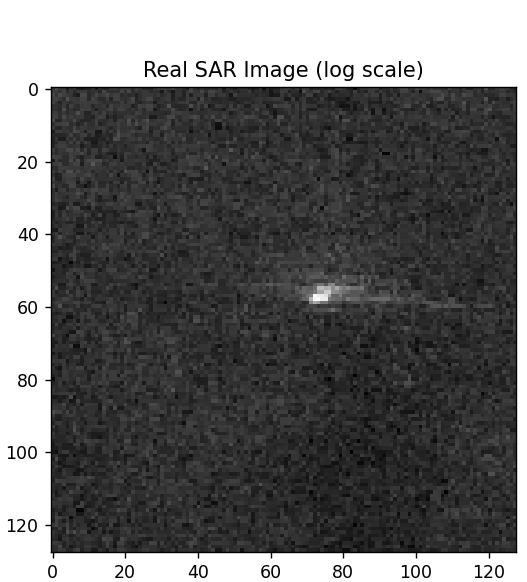
\includegraphics[width=0.6\textwidth, height=0.4\textheight, keepaspectratio]{src/rapport_complet/img/detec_image_real1.png}
    \caption{Image réelle coupée (128x128) avant application de l'algorithme de détection}
    \label{fig:visu_gain_approx_et_reel}
\end{figure}

\begin{figure}[H]
    \centering
    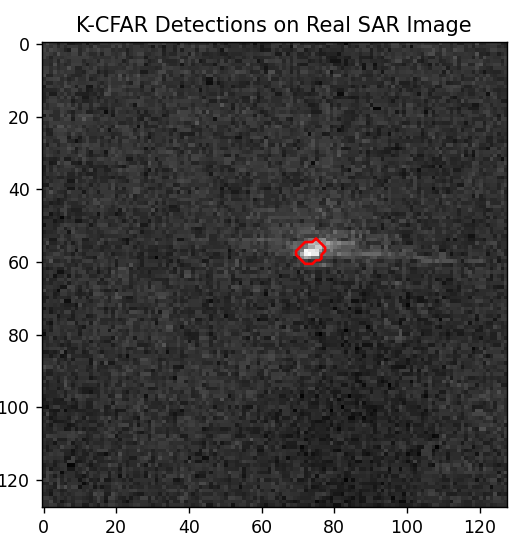
\includegraphics[width=0.6\textwidth, height=0.4\textheight, keepaspectratio]{src/rapport_complet/img/detec_image_real2.png}
    \caption{Image réelle coupée (128x128) après application de l'algorithme de détection}
    \label{fig:visu_gain_approx_et_reel}
\end{figure}


Les résultats obtenus montrent que l’algorithme est capable de détecter des zones d’intérêt tout en limitant les fausses alarmes, malgré la complexité du clutter réel.


\subsection{Conclusion}

L’algorithme K-CFAR implémenté permet de réaliser une détection robuste dans les images SAR en tenant compte des propriétés statistiques du clutter. L’adaptation locale du seuil garantit une maîtrise de la probabilité de fausse alarme, tandis que les traitements de post-filtrage améliorent la qualité des détections.

L’ensemble de ces résultats valide l’intégration de cet algorithme dans la chaîne globale de traitement SAR.